\chapter{Theoretische Grundlagen}


\section{Siliziumdetektoren}

Die im Silizium vorkommenden Elektronen wechselwirken mit anderen Elektronen und
Kernen des Kristalls, wodurch es zu vielen Aufspaltungen des Energieniveaus der Elektronen kommt. Durch das Pauli-Prinzip können
die Elektronen nicht dieselben Quantenzahlen besitzen, wodurch sich deren Energieniveaus voneinander unterscheidet.
Die Zustände liegen dicht bei einander, weshalb von Energiebändern gesprochen wird.
Das Höchste von den Elektronen besetzte Band im Grundzustand ist das Valenzband, welches von dem
nächsthöheren Band durch eine Bandlücke getrennt ist. Elektronen können
durch Anregungen in das Leitungsband wandern und somit Strom leiten, vorausgesetzt
die Anregungen sind größer als die Energielücke.

Das Einbringen von Fremdatomen in den Siliziumkristall kann dessen Eigenschaften ändern
und wird Dotierung genannt.
Hat das Fremdatom mehr oder weniger Valenzelektronen als das Silizium, ersetzt ein neuer Zustand innerhalb der Bandlücke
einen alten Zustand.
Bei den Fremdatomen wird zwischen Donatoren und Akzeptoren unterschieden, wobei die
Ersteren mehr Valenzelektronen als das Silizium besitzen und die Zweiteren weniger.
Durch Donatoren wird es für Elektronen einfacher in das Leitungsband zu wandern. Akzeptoren
erschaffen ein Loch über dem Valenzband, welches durch ein Elektron gefüllt wird und somit ein
Loch im Valenzband zurückbleibt.
Bereiche des Siliziumkristalls mit Donatoren werden n-Dotierte Bereiche
und mit Akzeptoren p-Dotierte Bereiche genannt.

Bei einem Übergang von einer n-Dotierten zu einer p-Dotierten Schicht rekombinieren die durch
thermische Anregung entstehenden freien Ladungsträger
der n-und p-Dotierten Schicht, da beide
in die anderen Bereiche diffundieren. Die Diffusion findet aufgrund der Dotierung und die dadurch folgenden unterschiedlichen
Konzentrationen von Elektronen und Löchern der beiden Bereiche statt.
Durch die übrig bleibenden ortsfesten Atomkerne
baut sich ein elektrisches Feld auf, welches dem Diffusionsstrom entgegenwirkt.
Ein sich einstellendes Gleichgewicht führt zu einer ladungsträgerfreien Zone bei
9m Bereich des p-n-Übergangs.
Für Detektoren werden die Bereiche von Bulk und Oberfläche unterschiedlich stark dotiert, wobei typischerweise eine starke n-und
p-dotierte Oberfläche und ein leicht dotierter Bulk verwendet wird. Durch die asymmetrische
Dotierung breitet sich die Depletionszone hauptsächlich in den schwächer dotierten Bulk aus.
Im Falle von ($N_{\mathrm{A}} \gg N_{\mathrm{D}}$) lässt sich die Depletionstiefe $d$ beschreiben durch:
\begin{align}
  d \approx \sqrt{\frac{2 \epsilon \epsilon_0}{e} (U_{\mathrm{bi}}+U_{\mathrm{ext}})\frac{1}{N_{\mathrm{D}}}}.
  \label{eqn:depletionsdicke}
\end{align}
Hierbei beschreibt $\epsilon \epsilon_0$ die Permittivität, $e$ die Elementarladung, $N_{\mathrm{D}}$ die Donatorenkonzentration, $U_{\mathrm{bi}}$ (\textit{built-in voltage})  die
durch die festen Raumladungen entstehende Spannung und $U_{\mathrm{ext}}$ die extern angelegte Spannung. Für ideale Detektoren gilt $N_{\mathrm{D}} = N_{\mathrm{eff}}$, bei
strahlengeschädigten Detektoren ist dies nicht mehr der Fall, wodurch in Gleichung \ref{eqn:depletionsdicke} das $N_{\mathrm{D}}$ durch $N_{\mathrm{eff}}$ ersetzt werden muss.


Durch eine äußere negative Spannung  an der p-Seite in Bezug zur n-Seite wird die Zone vergrößert und dient als Ionisationskammer für einfallende Teilchen. Diese streuen vor allem
an den Elektronen der Atome in der Zone und geben ein Teil oder ihre gesamte Energie bei dem Durchgang durch den Detektor ab. Mit der so abgegebenen
Energie werden Elektron-Loch Paare erzeugt, welche sich durch das vorhandene elektrische Feld zu ihrer jeweiligen dotierten
Schicht bewegen und über Elektroden als elektrisches Signal gemessen werden können. Des Weiteren ist die Depletionszone essenziell damit
die entstehenden Elektron-Loch Paare nicht mit vorhandenen Ladungsräger rekombinieren, was zu einer deutlichen Verringerung des Signales führen würde.
Die ladungsträgerfreie Zone fungiert somit als Detektor und soll ein möglichst großes Volumen umfassen.

Mehr Informationen über Detektoren finden sich in  \cite{semiconductor}.

\section{Strahlenschäden}
Wechselwirkungen von Teilchen mit Silizium können zu Defekten in deren
Gitterstruktur führen.
Die Energie der Teilchen wird dabei durch Ionisation und elastischer Streuung mit den Atomkernen abgegeben. Über Ionisation abgegebene Energie
fließt dabei in die
\textit{Total Ionizing Dose} (TID) ein und führt zu keinen Schäden im Bulk, lediglich das Streuen der Strahlung an den
Atomkernen kann zu Defekten im Gitter führen.

Es muss zwischen verschiedenen Arten von Defekten unterschieden werden. Die Teilchen können ein Gitteratom aus dem
Gitter herausschlagen, wodurch eine Leerstelle und ein Zwischengitteratom entstehen. Das herausgeschlagene Atom
kann Silizium, aber auch ein Fremdatom sein. Daraus folgt eine Änderung der Dotierungskonzentration im
Halbleiter und somit eine Änderung seiner Eigenschaften. Zum Beispiel können neue Zustände nahe der Mitte der
Bandlücke entstehen, welche Elektronen und Löcher aus dem Valenzband einfangen  und in das Leitungsband
abgeben, wodurch der Leckstrom wächst.


Die durch Strahlenschäden hervorgerufenen Energiezustände verhalten sich hauptsächlich wie Akzeptoren im Siliziumgitter. Bei
einer steigenden Anzahl an Defekten wächst die p-Dotierung der Schichten. Für die n-dotierte Schicht kann
es zur sogennanten Typinversion kommen, wodurch diese sich in eine leicht p-dotierte Schicht umwandelt. Bei einer
solchen Typinversion
geht die benötigte externe Spannung wegen \ref{eqn:depletionsdicke} für das Depletieren des Sensors,
sowie die Dotierungskonzentration gegen null.
Für größer werdende Fluenzen steigt die benötigte externe Spannung und die
Dotierungskonzentration wieder kontinuierlich an.
In Abbildung \ref{fig:typeinversion} ist eine Typinversion aus \cite{typinversion} dargestellt.

\begin{figure}
  \centering
    \includegraphics[width=0.82\textwidth]{build/typeinversion.PNG}
\caption{Depletionsspannung und Dotierungskonzentration in Abhängigkeit von der Fluenz \cite{typinversion}.}
\label{fig:typeinversion}
\end{figure}

Gemäß der \textit{Non-Ionizing Energy Loss} (NIEL) Hypothese ist der entstehende Schaden des Detektors durch
herausgeschlagene Atome des Gitters proportional zur Energie, welche durch Streuung an die Zwischengitteratome abgegeben wird.
Abhängig von der Energie des Zwischengitteratoms kann dieses weitere Atome aus dem Gitter schlagen und somit
eine Kaskade von Defekten auslösen. Der dem Detektor zugefügte Schaden ist dabei
lediglich abhängig von der abgegeben Energie und nicht vom Verlauf der Kaskade und dem Stoßpartner.
Um somit Fluenzen $ \Phi$ von verschiedenen Teilchen (Lepton, Hadron) miteinander vergleichen zu können, werden diese
auf dne NIEL einer $\SI{1}{\mega\eV}$ Neutronstrahlung normalisiert und haben die Einheit $[\Phi_{\mathrm{eq}}]=\mathrm{n_{\mathrm{eq}}/cm^2}$.


\section{Annealing der Dotierungskonzentration}
Annealing beschreibt im Allgemeinen die durch Erhitzung hervorgerufenen Veränderungen von Materialeigenschaften. Für strahlengeschädigte
Halbleiter werden dabei, durch die zugeführte Wärme, die Defekte teilweise behoben, um somit eine
bessere Funktionsfähigkeit über einen längeren Zeitraum zu garantieren. Die auftretenden Effekte sind dabei wie folgt:

\textbf{1. Migration:} Ist die Temperatur hoch genug können die Zwischengitteratome durch das Gitter wandern und
Leerstellen im Gitter füllen.

\textbf{2. Komplexformation:} Das Migrieren der Atome kann zum Ausbilden von Komplexen führen. Dies geschieht durch das
Gruppieren von mehreren Zwischengitteratomen im Kristall.

\textbf{3. Dissoziation:} Komplexe und Fehlstellen können bei hohen Temperaturen dissoziieren, wodurch einzelne Bestandteile des Komplexes
durch das Gitter migrieren können. Dafür muss die Schwingungsenergie des Gitters größer als die Bindungsenergie der Komplexe sein.
Zwischengitteratome können jedoch auch stabile Komplexe miteinander bilden.
Diese werden nicht durch Annealing
beeinflusst und verändern die Halbleiter permanent.

Die Bestrahlung und die Annealingeffekte bewirken eine Änderung in der effektiven Dotierungskonzentration
${N_{\mathrm{eff}}= |N_{\mathrm{D}}-N_{\mathrm{A}}|}$,
welches durch das Hamburger Modell beschrieben wird.
Die Änderung von $N_{\mathrm{eff}}$ ist gegeben durch:
\begin{align}
  \Delta N_{\mathrm{eff}}(t, \Phi_{\mathrm{eq}}, T)   = N_{\mathrm{C}}(\Phi_{\mathrm{eq}}) + N_{\mathrm{A}}(t, \Phi_{\mathrm{eq}}, T) + N_{\mathrm{Y}}(t, \Phi_{\mathrm{eq}}, T) \text{\cite{moll}}
  \label{eqn:N_eff}
\end{align}
Die einzelnen Summanden werden im folgenden erläutert.

\textbf{\textit{Stable Damage}} $\symbf{N_{\mathrm{C}}}:$ Der stable Damage wird durch Annealing nicht beeinflusst.
\begin{align}
  N_{\mathrm{C}}(\Phi_{\mathrm{eq}}) = N_{\mathrm{C0}}[1-\exp{(-c \cdot \Phi_{\mathrm{eq}})}] + g_{\mathrm{c}} \cdot \Phi_{\mathrm{eq}}
\end{align}
Der erste Summand beschreibt wie die Anzahl an Donatoren mit
steigender Fluenz asymptotisch gegen 0 gehen, der zweite Summand beschreibt stabile Defekte, welche sich wie Akzeptoren verhalten \cite{beyer}.
Hierbei beschreibt $N_{\mathrm{C0}}$ die entfernte Donatorenkonzentration, $g_{\mathrm{c}}$ die sogenannte \textit{introduction rate} der Akzeptoren und $c$ einen Fitparameter.
Die \textit{introduction rate} beschreibt die Anzahl an durch Bestrahlung entstehenden Akzeptoren.

\textbf{\textit{Shortterm annealing}} $\symbf{N_{\mathrm{A}}}:$ Das shortterm Annealing bewirkt eine Verringerung der Dotierungskonzentration und entsteht durch
das Annealing von Akzeptoren, was zu einer kleineren Dotierungskonzentration führt. Dieser Effekt wird beim
gezielten Ausheilen des Sensors ausgenutzt. Die Bezeichnung rührt daher, dass $N_{\mathrm{A}}$ meistens in den ersten 100 Minuten verschwindend gering wird. Die
Funktion wird näherungsweise beschrieben durch:
\begin{align}
  N_{\mathrm{A}}(t, \Phi_{\mathrm{eq}}, T) = \Phi_{\mathrm{eq}} \cdot g_{\mathrm{a}} \cdot \exp{\left(-\frac{t}{\tau_{\mathrm{a}}(T)}\right)}.
\end{align}
Hierbei gilt für die temperaturabhängige Funktion
\begin{align}
  \tau_{\mathrm{a}}(T) = \frac{1}{k_{0\mathrm{a}}}\exp{\left(\frac{E_{aa}}{k_{\mathrm{b}}T}\right)},
\end{align}
Mit der \textit{introduction rate} $g_{\mathrm{a}}$, dem Frequenzfaktor $k_{0\mathrm{a}}$, der Boltzmann Konstante $k_{\mathrm{b}}$ und
der Aktivierungsenergie $E_{aa}$. Die Aktivierungsenergie beschreibt dabei die nötige Energie für das Ausheilen der Defekte.
Der Frequenzfaktor ist im Bereich der am häufigsten auftretenden Phononenfrequenz ${f = k_{\mathrm{B}}T/h \approx \SI{10e13}{\per\second}}$, wodurch
die betroffenen Defekte höchstwahrscheinlich durch Dissoziation ausheilen, da dieser ein Prozess mit einer einzelnen Zustandsänderung ist.


\textbf{\textit{Longterm annealing}} $\symbf{N_{\mathrm{Y}}}:$ Der Aufbau von
Akzeptoren sorgen nach einem hinreichend großen Zeitraum für eine steigende
Dotierungskonzentration. Dieser Effekt wird wie folgt berechnet.
\begin{align}
  N_{\mathrm{Y}}(t, \Phi_{\mathrm{eq}}, T)     = \underbrace{N_{\mathrm{Y , \inf}}}_{g_{\mathrm{Y}}\cdot\Phi_{\mathrm{eq}}}\cdot \left(1 - \frac{1}{1 + \frac{t}{\tau_{\mathrm{Y}}(T)}}\right)
\end{align}
Beginnend bei null läuft die Funktion asymptotisch gegen die Konstante $N_{\mathrm{Y, \inf}}$.
Für $\tau_{\mathrm{Y}}(T)$ gilt:
\begin{align}
  \tau_{\mathrm{Y}}(T) = \frac{1}{k_{0\mathrm{Y}}}\exp{\left(\frac{E_{Y}}{k_{\mathrm{b}}T}\right)}.
\end{align}
Auch hier ist $k_{0\mathrm{Y}}$ ein Frequenzfaktor und $E_{\mathrm{Y}}$ die Aktivierungsenergie. Der Faktor $N_{\mathrm{Y , \inf}}$
ist das Produkt der \textit{introduction rate} $g_{\mathrm{Y}}$ und der Fluenz.
In Abbildung \ref{fig:n_eff_beispiel} ist beispielhaft die Änderung der Dotierungskonzentration mit Annealing eines
Sensors dargestellt.

\begin{figure}
  \centering
  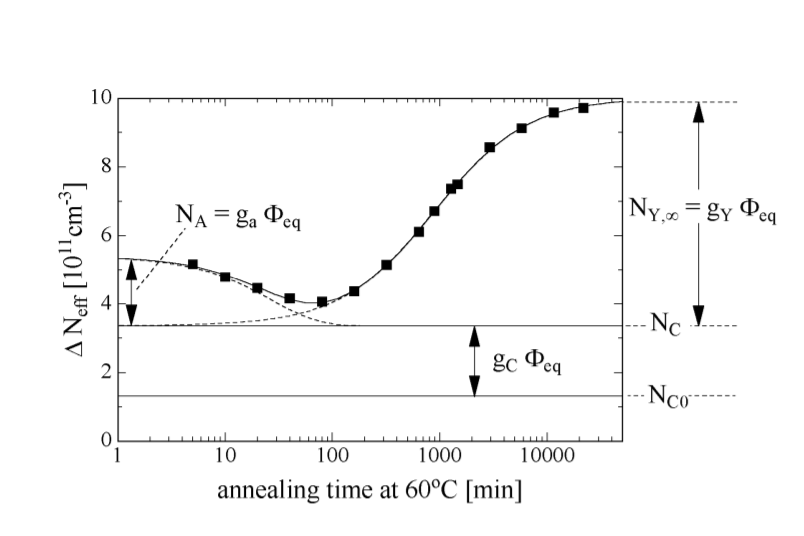
\includegraphics[width=0.82\textwidth]{logos/n_eff_beispiel.PNG}
  \caption{Dotierungskonzentration bei 60°C für eine Bestrahlung mit einer Fluenz von
  $1,4\cdot 10^{13} \, \mathrm{n_{eq}/cm^2}$.\cite{moll}}
  \label{fig:n_eff_beispiel}
\end{figure}



\section{Annealing des Leckstroms}
Der Leckstrom beschreibt allgemein einen messbaren Stromfluss über einen als isolierend
angenommenen Weg. Bei den hier thematisierten Sensoren ist damit der Strom gemeint, der trotz sperrender
Diode fließt. Dieser entsteht hauptsächlich durch die Generation von Ladungsträgern an Defekten, welche
bei realen Dioden auch vor der Bestrahlung vorhanden sind. \cite{moll}.
Durch das Annealing werden die Defekte in der Mitte der Energielücke teilweise behoben,
was zu einer Verringerung des Leckstroms führt.

Der Leckstrom vor und nach der Bestrahlung ist temperaturabhängig und wird
beschrieben durch
\begin{align}
  I(T) \propto T^2 \exp{\left(\frac{-E_{\mathrm{eff}}}{2 k_{\mathrm{B}}T}\right)} \text{\cite{Chilingarov_2013}} \label{eqn:Chilingarov_2013}.
\end{align}
Hierbei ist $E_{\mathrm{eff}}$ die  effektive Aktivierungsenergie. Mmehr Information in \cite{Chilingarov_2013}.

Die Fluenz und der durch Strahlung hervorgerufene Leckstrom $\Delta I$ sind
proportional zueinander:


\begin{align}
  \Delta I = \alpha \Phi_{\mathrm{eq}} \cdot V .
\end{align}
Hierbei ist $V$ das Volumen des Detektormaterials und $\alpha$ die
sogenannte Schadensrate.



Die Verringerung des Leckstromes durch Annealing wird mit der Schadensrate
beschrieben, welche als eine Funktion abhängig von der Zeit und
Temperatur beschrieben wird.\cite{moll}

\begin{align}
  \alpha(t, T) = \underbrace{\alpha_I \cdot \exp{\left(-\frac{t}{\tau_{\mathrm{I}}(T)}\right)}}_{\mathrm{shortterm \: annealing}} + \underbrace{\alpha_{\mathrm{0}}(T) -\beta \cdot \ln{\left(\frac{t}{t_{\mathrm{0}}}\right)}}_{\mathrm{longterm \: annealing}} \text{\label{eqn:damage}}
\end{align}
Hierbei sind $\alpha_I$, $\beta$ und $\alpha_{\mathrm{0}}(T)$ Fitparameter und $\tau_{\mathrm{I}}(T)$ eine
temperaturabhängige Funktion:
\begin{align}
  &\alpha_{\mathrm{0}}(T) = \SI{-8.9e-17}{\ampere\per\centi\meter} + \SI{4.6e-14}{\ampere\kelvin\per\centi\meter} \cdot \frac{1}{T} \\
  &\tau_{\mathrm{a}}(T) = \frac{1}{k_{0\mathrm{I}}}\exp{\left(\frac{E_{I}}{k_{\mathrm{B}}T}\right)}
\end{align}
Wie für $N_{\mathrm{A}}$ und $N_{\mathrm{Y}}$ ist $k_{0\mathrm{I}}$ ein Frequenzfaktor und $E_{I}$ die Aktivierungsenergie.

Anders als das Annealingverhalten der Dotierungskonzentration kann die Schadensrate
bei fortschreitendem Annealing nur sinken. Für kurze und
lange Zeiten dominieren in diesem Modell wie bei der Dotierungskonzentration unterschiedliche
Terme. Für große Temperaturen und Zeiten würde $\alpha$ kleiner als null
werden, was unphysikalisch wäre.
Die Messwerte für kleine Schadensraten weichen jedoch von den
Vorhersagen des Modells ab und nähern sich einen Wert größer null an. Das Modell versagt in diesem Fall.
Dies ist in Abbildung \ref{fig:damage_rates} dargestellt.

\begin{figure}
  \centering
  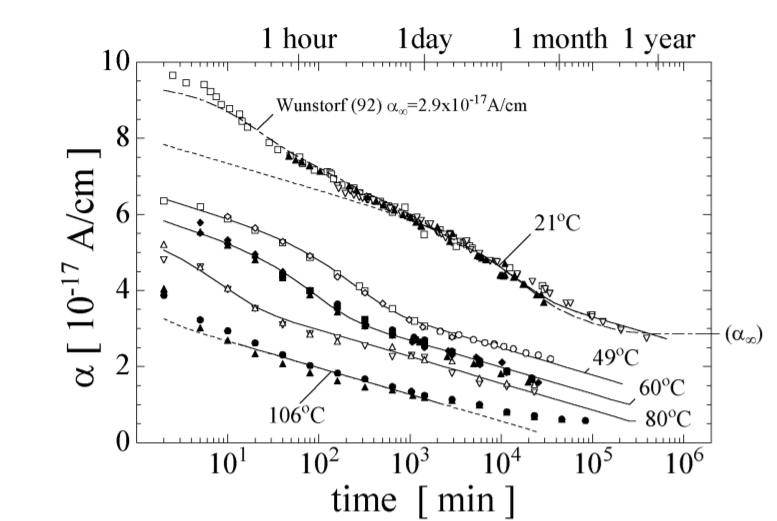
\includegraphics[width=0.82\textwidth]{logos/schadensraten.PNG}
  \caption{Schadensraten für verschiedene konstante Annealingtemperaturen.\cite{moll}}
  \label{fig:damage_rates}
\end{figure}
